
\documentclass[a4paper,12pt]{article}

\usepackage{indentfirst}
\usepackage{cite}
\usepackage[utf8]{inputenc}
\usepackage[T1]{polski}
\usepackage{helvet}
\usepackage{graphicx}
\usepackage{svg}
\usepackage{color}
\usepackage{geometry}
\usepackage{float}
\usepackage{multirow}
\usepackage[hidelinks]{hyperref}
\usepackage{caption}
% dodaj bibliografię do spisu treści
\usepackage[nottoc]{tocbibind}
% unikaj pojedynczych linii na początku/ końcu stron
\usepackage[defaultlines=4,all]{nowidow}
\usepackage{subcaption}
\usepackage{minted}
\usepackage{amsmath}
\usepackage{amsfonts}

% set default figure placement to !htbp
\makeatletter
\def\fps@figure{!htbp}
\makeatother


\setminted{ frame=lines,
framesep=2mm,
baselinestretch=1.2,
fontsize=\footnotesize,
linenos
}

\newcommand{\setSubtitle}[1]{
    \newcommand{\subtitle}{#1}
    }


\title{Ochrona przed korozją i erozją materiałów budowlanych}
\setSubtitle{\small{Sprawozdanie z badań wykwitów solnych}}
\author{Aleksandra Barcz \newline Alicja Kotwica \newline Gabriela Rojek}
\date{\today}


\makeatletter
\newcommand{\linia}{\rule{\linewidth}{0.4mm}}
\renewcommand{\maketitle}{\begin{titlepage}
    \begin{figure}[!htbp]
      \centering
      
\includegraphics{img/logoAGH}
    \end{figure}
    \vspace*{1cm}
    \begin{center}\small
    Akademia Górniczo -- Hutnicza\\
    Wydział Inżynierii Materiałowej i Ceramiki
    \end{center}
    \vspace{2cm}
    \noindent\linia
    \begin{center}
      \LARGE \textsc{\@title}
    \end{center}
            \begin{center}
      \large \textsc{\subtitle}
      \end{center}     
     \linia
    \vspace{0.5cm}
    \begin{flushright}
    \begin{minipage}{5cm}
    \textit{\small Autorzy:}\\
    \normalsize \textsc{\@author} \par
    \end{minipage}
    \vspace{4cm}
     \end{flushright}
    \vspace*{\stretch{6}}
    \begin{center}
    \@date
    \end{center}
  \end{titlepage}%
}
\makeatother

\begin{document}
\maketitle
{
\setcounter{tocdepth}{3}
\pagenumbering{roman} 
%\tableofcontents
\newpage
\pagenumbering{arabic} 
}

\section{Obecność szkodliwych soli rozpuszczalnych.}

\subsection{Krótki opis przygotowania próbek do oznaczeń.}

Na początku roztopiliśmy parafinę, następnie przygotowane próbki umieściliśmy w osobnych pojemnikach. Pojemniki koniecznie muszą zostać umyte i przepłukane wodą destylowaną w celu usunięcia alkaliów. Próbki zostały postawione pionowo na środku pojemnika i zalane wodą. Natychmiast po wlaniu wody na powierzchnię tafli wylaliśmy roztopioną parafinę w taki sposób, aby pokryła dokładnie całą taflę wody. Woda nie może mieć dostępu do powietrza, żeby nie wyparowała.

\subsection{Przeprowadź oględziny poszczególnych próbek po badaniu. Obecność wykwitów, położenie, kolor, ilość, usuwalność - za pomocą ostrego narzędzia.}

\begin{description}
    \item[A] Opis próbek zawierających siarczan magnezu
    \newline
    \newline
    Wykwity w tej próbce pojawiły się tylko na jednej płytce, na jej samym czubku w rogu materiału. Mają one kolor biały, występują w niedużej ilości i prawdopodobnie są trudno usuwalne ostrym narzędziem.

    \begin{figure}[H]
        \begin{center}
        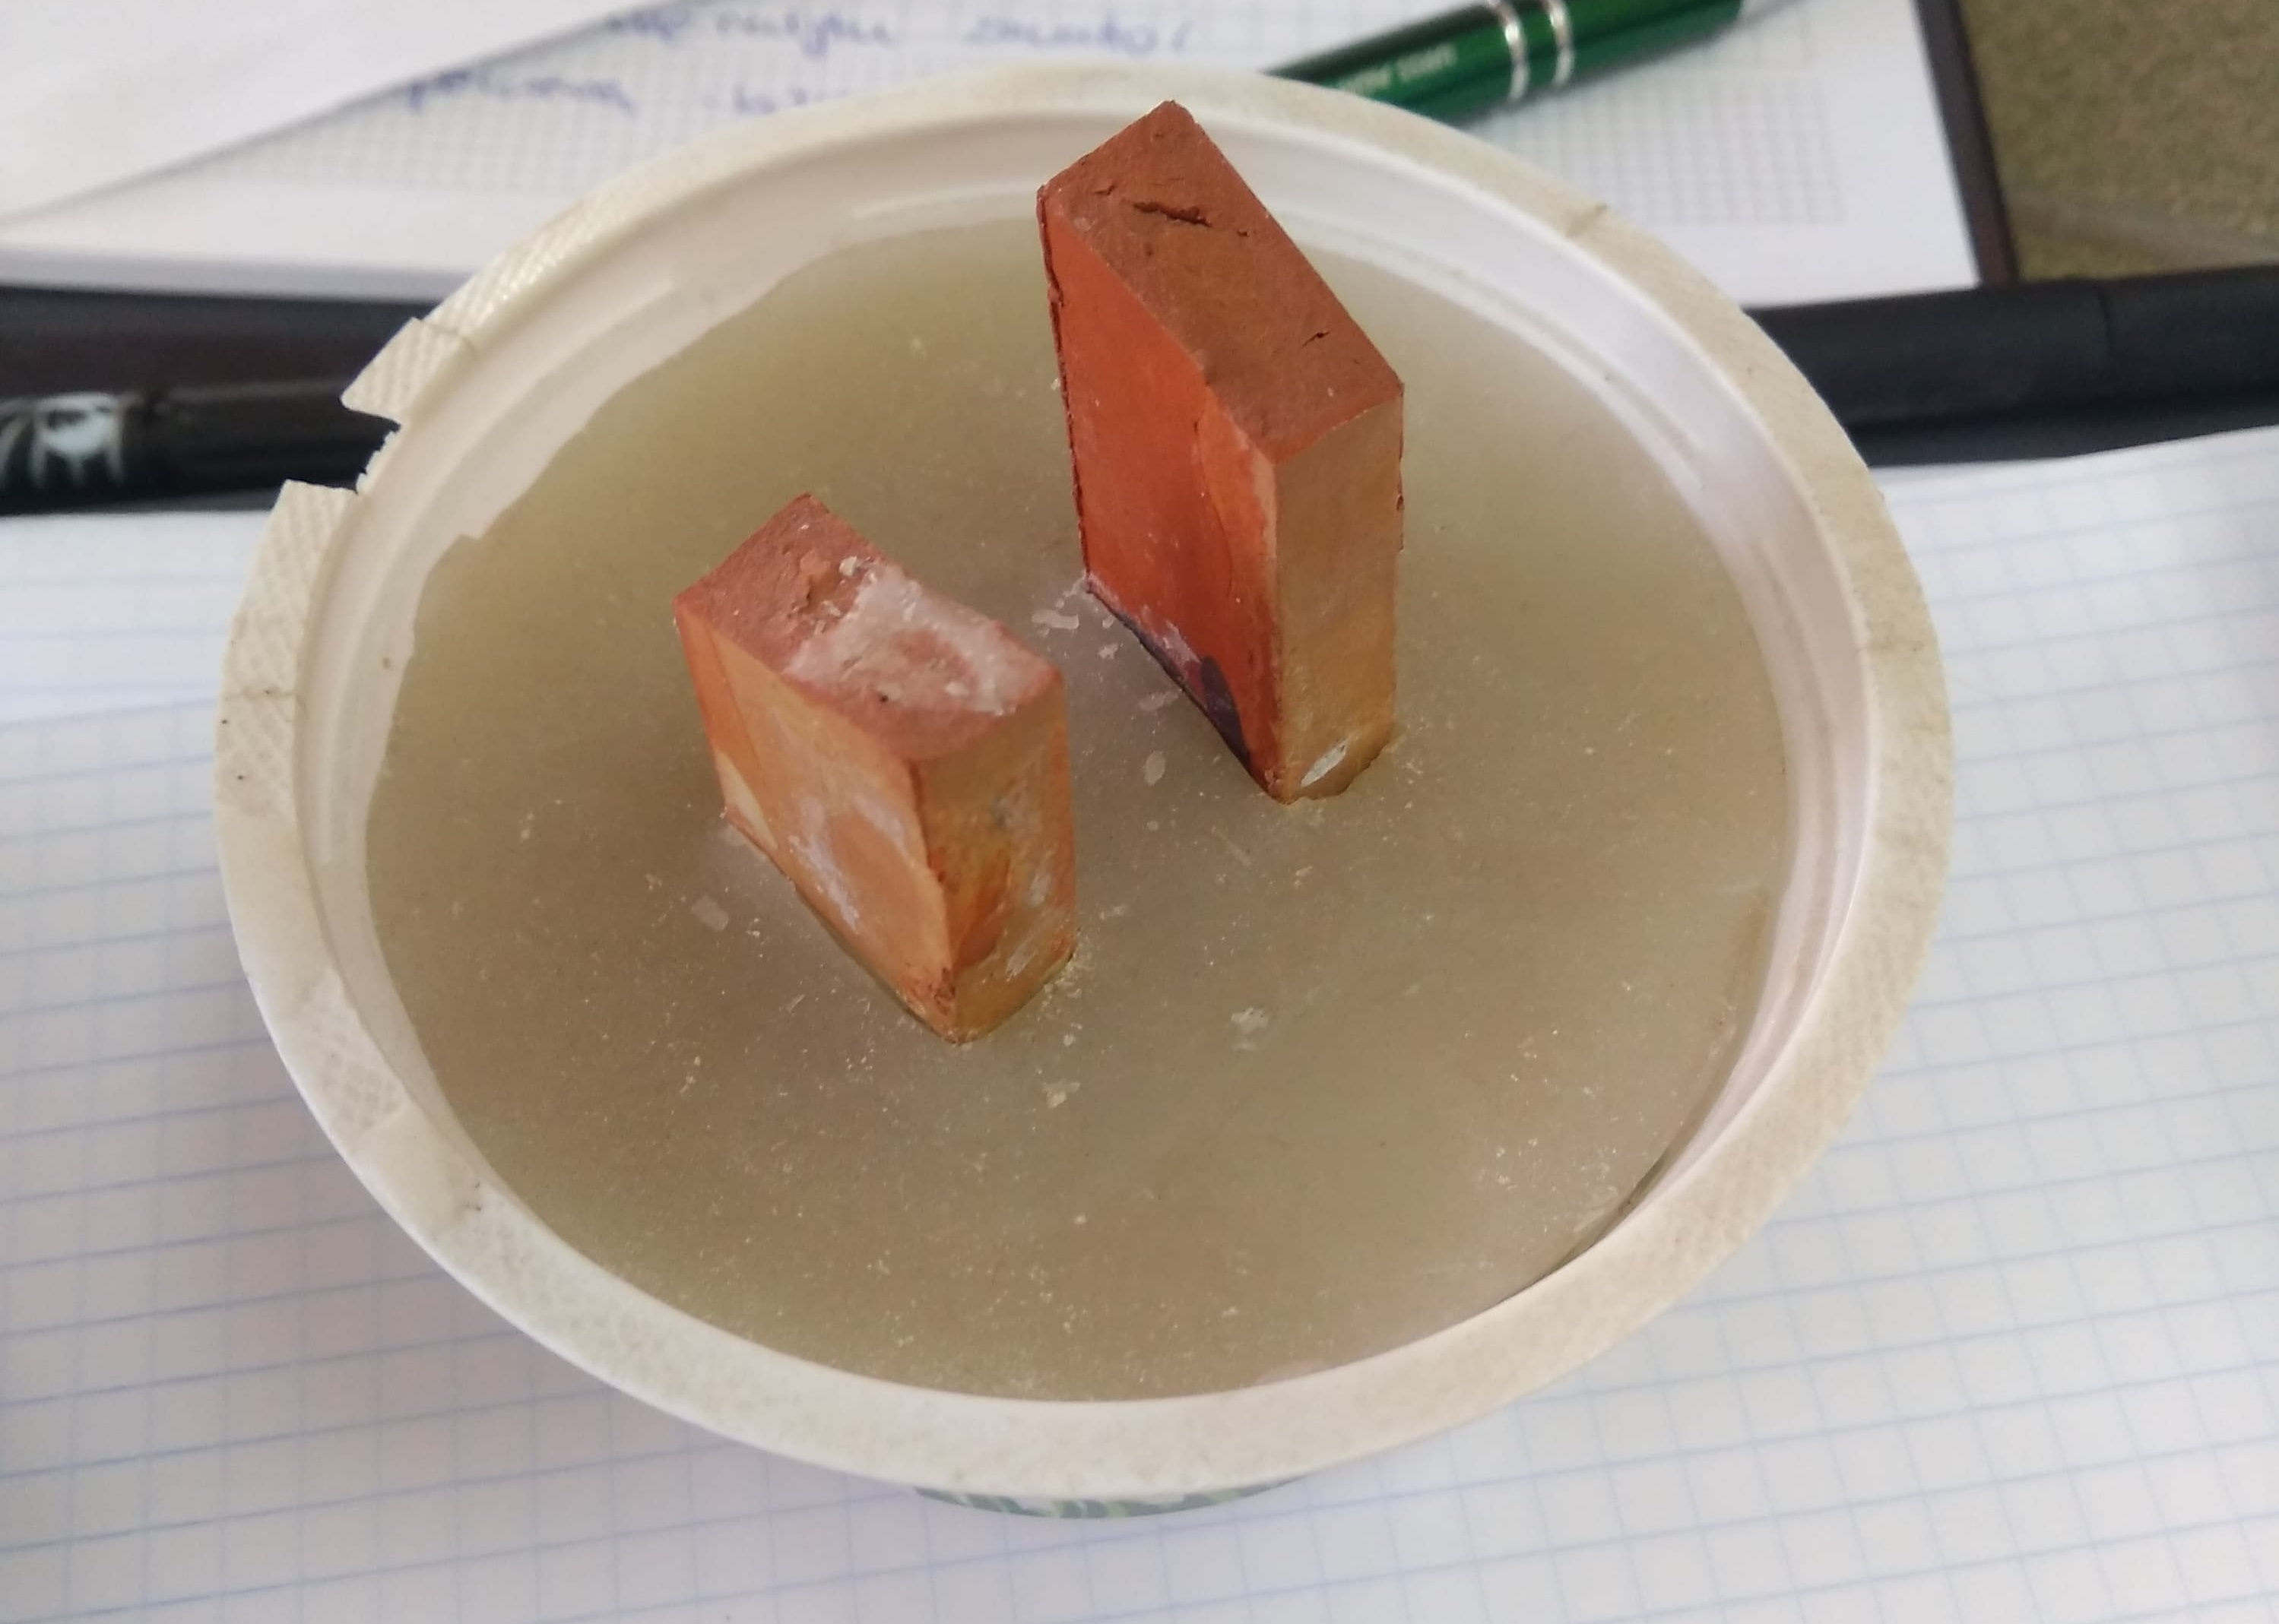
\includegraphics[width=0.7\textwidth]{img/siarczan_magnezu.jpg}
        \caption{Próbka siarczanu magnezu.}
        \end{center}
    \end{figure}

    \item[B] Opis próbek zawierających siarczan sodu 
    \newline
    \newline
    Wykwity w tej próbce pojawiły się na obu płytkach, w ich górnych częściach od tej samej strony. Mają one kolor biały, występują w znacznej ilości i prawdopodobnie są łatwo usuwalne ostrym narzędziem.

    \begin{figure}[H]
        \begin{center}
            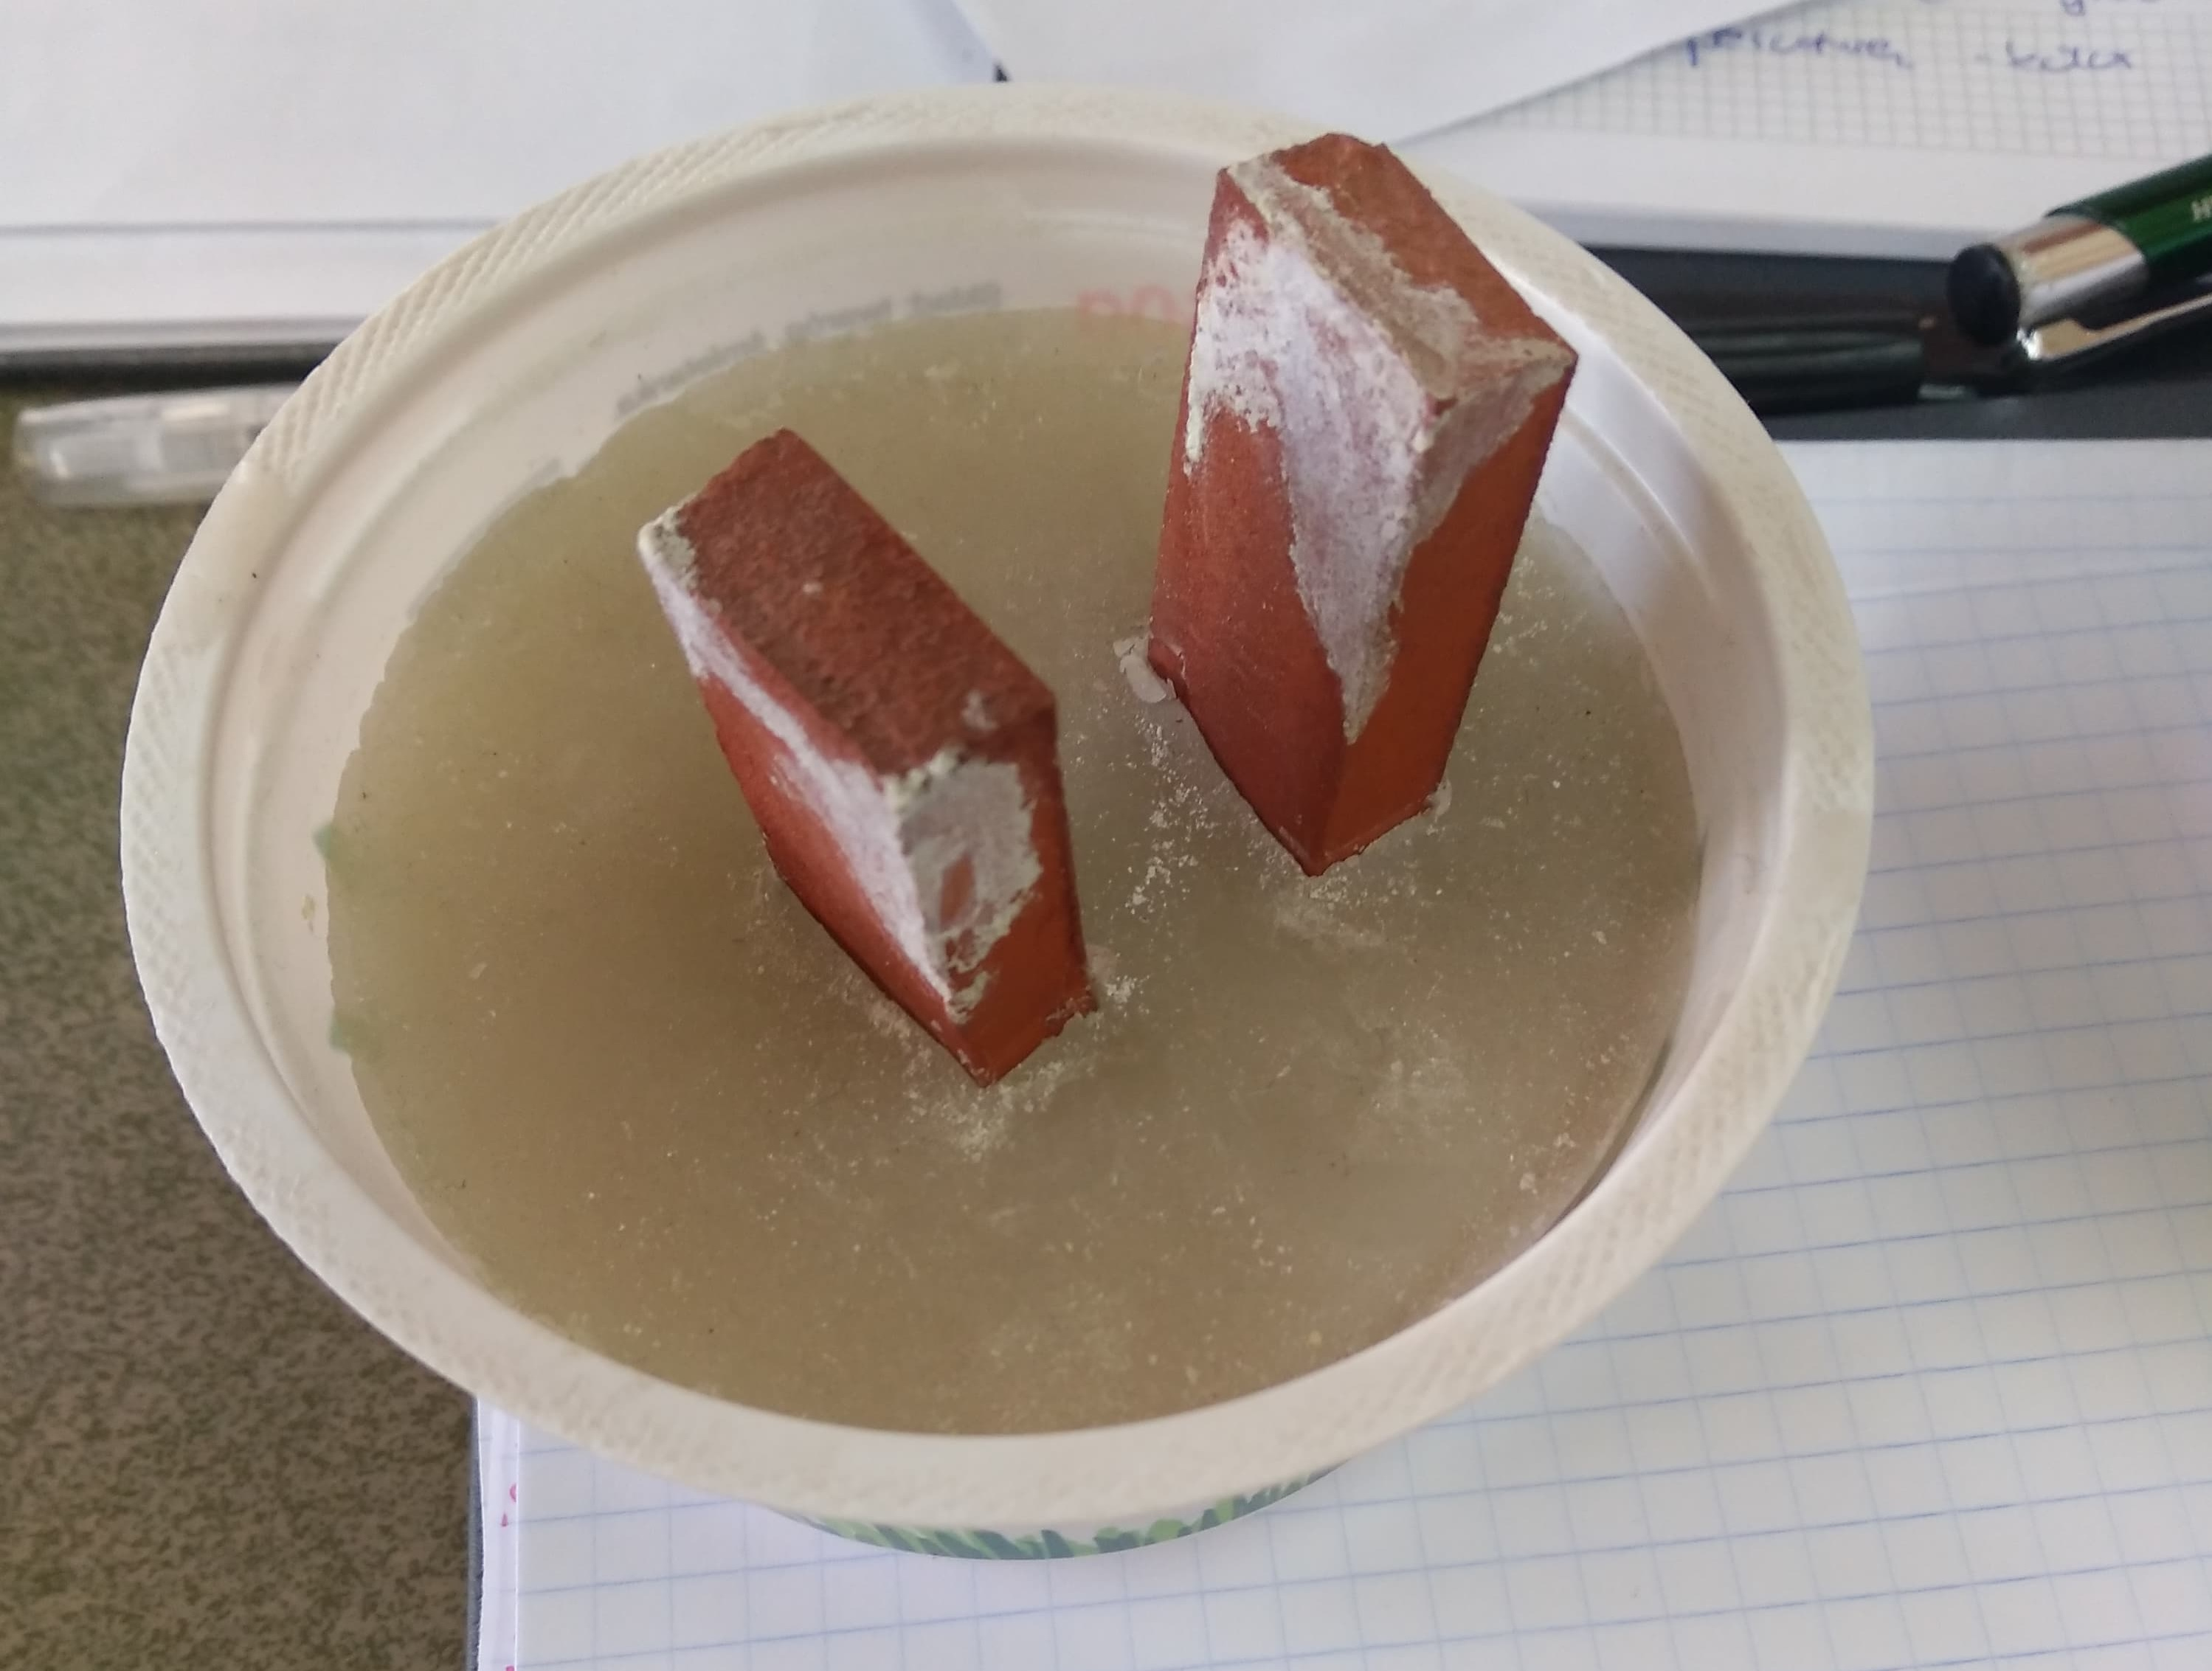
\includegraphics[width=0.7\textwidth]{img/siarczan_sodu.jpg}
            \caption{Próbka siarczanu sodu.}
        \end{center}
    \end{figure}

\end{description}

\subsection{Wnioski z przeprowadzonych badań z części $1$.}

Umiejscowienie wykwitów jest takie, a nie inne, ponieważ w tym miejscu występuje najbardziej intensywne parowanie. Jest to miejsce krystalizacji. Siarczan sodu oraz ogólnie alkalia, wpływają na proces wypalania materiału, przez co próbka w nim zanurzona ma ciemniejszy odcień.

\newpage

\section{Obecność szkodliwego marglu.}



\subsection{Krótki opis sposobu naparzania próbek.}

Próbki dajemy na sito, które umieszczamy na garnku z gotującą się wodą. Wykorzystujemy tę metodę, ponieważ para wodna ma większą wnikliwość w porównaniu do wody, co oznacza, że spenetruje ona więcej porów.

\subsection{Przeprowadź oględziny poszczególnych próbek po badaniu. Oceń poziom i rodzaj ewentualnych zniszczeń spowodowanych obecnością węglanów w surowcu.}

\begin{description}
    \item[A] Próbki G1 ($1\%$ kamienia wapiennego o uziarnieniu powyżej $1mm$ w surowcu ilastym)
    \newline
    \newline
    Na powierzchni próbki możemy zauważyć niewielką ilość kamienia wapiennego, występującego w dużym uziarnieniu. Próbka posiadała duże spękania i ubytki.

    \begin{figure}[H]
        \begin{center}
            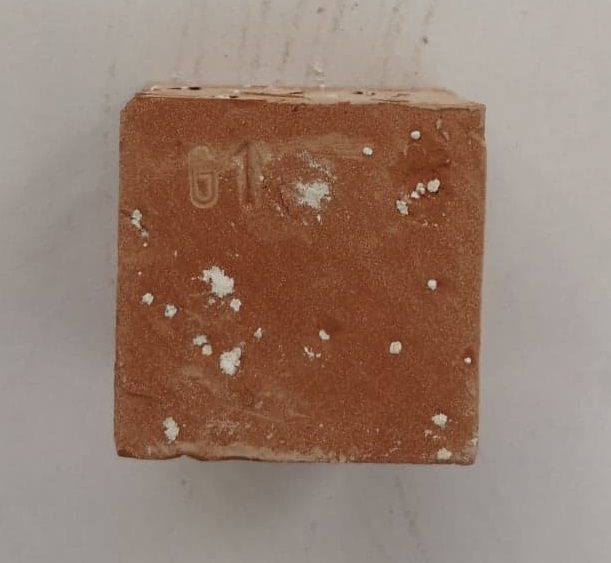
\includegraphics[width=0.5\textwidth]{img/G1.jpg}           
            \caption{Próbka G1 po naparzaniu.}
        \end{center}
    \end{figure}

    \newpage

    \item[B] Próbki D ($10\%$ kamienia wapiennego o uziarnieniu powyżej $0.5mm$ w surowcu ilastym)
     \newline
    Na powierzchni próbki możemy zauważyć większą ilość, drobniejszego kamienia wapiennego. Próbka nie posiadała większych spękań ani ubytków.

    \begin{figure}[H]
        \begin{center}
            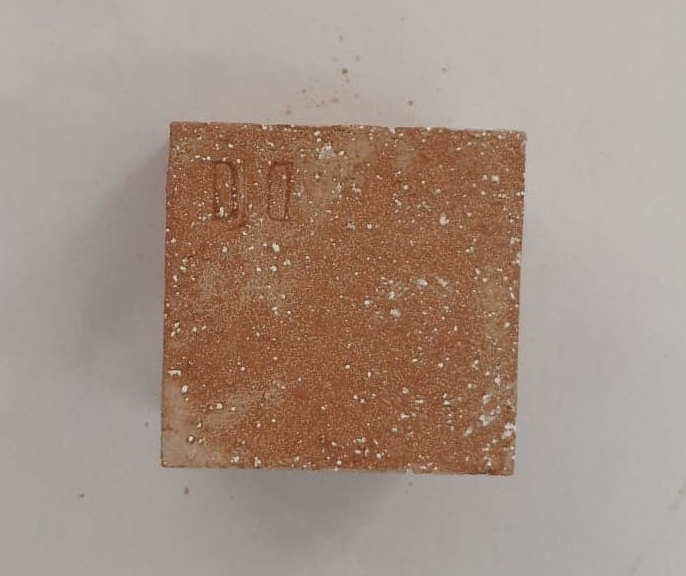
\includegraphics[width=0.5\textwidth]{img/D.jpg}           
            \caption{Próbka D po naparzaniu.}
        \end{center}
    \end{figure}

    \item[C] Próbki G10 ($10\%$ kamienia wapiennego o uziarnieniu powyżej $1mm$ w surowcu ilastym)  
    \newline
    Po naparzaniu próbka uległa całkowitemu rozpadowi na niewielkie 
    \newline
    kawałki, wśród których możemy dostrzec duże ziarna kamienia wapiennego. 

    \begin{figure}[H]
        \begin{center}
            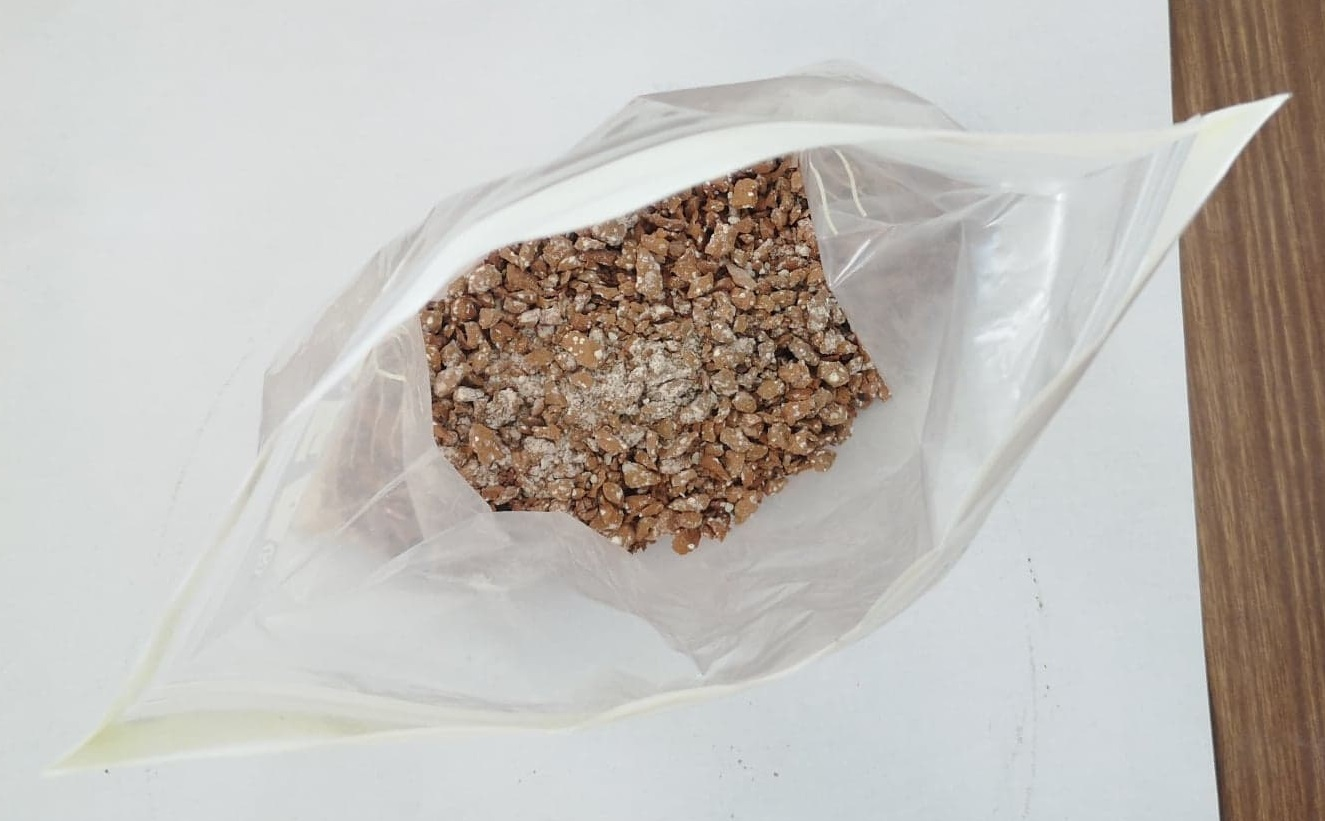
\includegraphics[width=0.7\textwidth]{img/G10.jpg}           
            \caption{Próbka G10 po naparzaniu.}
        \end{center}
    \end{figure}

\end{description}

\subsection{Wnioski z przeprowadzonych badań część $2$.}

Uszeregowanie próbek od najtrwalszej do najkruchszej:
\begin{itemize}
    \item D
    \item G1
    \item G10
\end{itemize}

Po jakości próbek możemy dojść do wniosku, że kamień wapienny znacząco pogarsza jakość próbki, zwłaszcza jeśli występuje on w dużym uziarnieniu i w dużej ilości. Jest to spowodowane faktem, iż pod wpływem wody i wilgoci margiel zwiększa swoją objętość. W rezultacie powoduje rozsadzenie materiału oraz powstanie dziur w próbce, co najlepiej obrazuje badana próbka G10.

% \bibliography{bibtex.bib}
% \bibliographystyle{unsrt}
\end{document}
